\documentclass[11pt]{article}
\usepackage[margin=1in]{geometry}
\usepackage{fontspec}
\usepackage{booktabs}
\usepackage{graphicx}
\usepackage[font=small,labelfont=bf]{caption}
\usepackage{natbib}
\usepackage{xurl}
\usepackage[hidelinks]{hyperref}
\usepackage{setspace}
\setstretch{1.12}
\newcommand{\BothN}{2065}
\newcommand{\DemCompatibility}{217}
\newcommand{\DemCompatibilityRate}{97.2}
\newcommand{\DemCompleted}{2023}
\newcommand{\DemDropout}{42}
\newcommand{\DemExcludedCI}{[-2.41, 0.37]}
\newcommand{\DemExcludedGap}{-1.02}
\newcommand{\DemExcludedOldRate}{97.4}
\newcommand{\DemExcludedOtherRate}{98.4}
\newcommand{\DemInstalledCI}{[-2.21, 0.55]}
\newcommand{\DemInstalledGap}{-0.83}
\newcommand{\DemInstalledOldRate}{97.4}
\newcommand{\DemInstalledOtherRate}{98.2}
\newcommand{\DemMissingP}{0.104}
\newcommand{\DemN}{2065}
\newcommand{\DemNoteP}{0.0499}
\newcommand{\DemOldP}{0.064}
\newcommand{\DemTokenCI}{[-2.33, 0.21]}
\newcommand{\DemTokenGap}{-1.06}
\newcommand{\DemTokenOldRate}{97.4}
\newcommand{\DemTokenOtherRate}{98.4}
\newcommand{\DemTruncated}{1405}
\newcommand{\DemUnknown}{14}
\newcommand{\FieldDates}{October 07 to October 14, 2009}
\newcommand{\HistoricalMissingGap}{0.411}
\newcommand{\HistoricalMissingN}{2013}
\newcommand{\JssN}{36,575}
\newcommand{\JssSurveys}{29}
\newcommand{\JulyCompleted}{1253}
\newcommand{\JulyExportN}{1296}
\newcommand{\JulyMissingAge}{9}
\newcommand{\JulyMissingParty}{11}
\newcommand{\JulyN}{1264}
\newcommand{\JulyUnfinished}{11}
\newcommand{\MergedColumns}{479}
\newcommand{\MergedN}{2330}
\newcommand{\MturkIncompleteN}{0}
\newcommand{\MturkN}{1133}
\newcommand{\PolCompatibility}{262}
\newcommand{\PolCompatibilityRate}{83.2}
\newcommand{\PolCompleted}{2069}
\newcommand{\PolDropout}{258}
\newcommand{\PolExcludedCI}{[-4.76, 0.75]}
\newcommand{\PolExcludedGap}{-2.01}
\newcommand{\PolExcludedOldRate}{88.5}
\newcommand{\PolExcludedOtherRate}{90.6}
\newcommand{\PolInstalledCI}{[-3.46, 1.98]}
\newcommand{\PolInstalledGap}{-0.74}
\newcommand{\PolInstalledOldRate}{88.5}
\newcommand{\PolInstalledOtherRate}{89.3}
\newcommand{\PolMissingP}{0.104}
\newcommand{\PolN}{2327}
\newcommand{\PolNoteP}{0.0082}
\newcommand{\PolOldP}{0.008}
\newcommand{\PolTokenCI}{[-5.93, -0.75]}
\newcommand{\PolTokenGap}{-3.34}
\newcommand{\PolTokenOldRate}{87.2}
\newcommand{\PolTokenOtherRate}{90.6}
\newcommand{\PolTruncated}{1587}
\newcommand{\PolUnknown}{19}
\newcommand{\UnderAgeN}{6}

\newcommand{\ChromeGap}{-0.41}
\newcommand{\ChromeInterval}{[-6.50, 1.13]}
\newcommand{\ChromeN}{72}
\newcommand{\ChromeOutsideN}{477}
\newcommand{\ChromeRate}{98.61}
\newcommand{\ChromeReferenceN}{715}
\newcommand{\ChromeReferenceRate}{99.02}
\newcommand{\CorpusUnknown}{141}
\newcommand{\JulyAnalysisN}{1,264}
\newcommand{\JulyDesktopMinutes}{3.0}
\newcommand{\JulyMobileMinutes}{3.1}
\newcommand{\LongRespondents}{628}
\newcommand{\LongRows}{5,652}
\newcommand{\LucidAnalysisN}{904}
\newcommand{\LucidDesktopMinutes}{5.5}
\newcommand{\LucidMetadataMissing}{171}
\newcommand{\LucidMobileMinutes}{5.1}
\newcommand{\LucidUnknownMinutes}{1.5}
\newcommand{\MarchAnalysisN}{1,060}
\newcommand{\MarchDesktopMinutes}{8.3}
\newcommand{\MarchMobileMinutes}{7.6}
\newcommand{\ParserAgreement}{532}
\newcommand{\ParserDifferent}{18}
\newcommand{\ParserMissing}{171}
\newcommand{\ParserUnresolved}{183}
\newcommand{\ResolutionGap}{-0.51}
\newcommand{\ResolutionInterval}{[-6.44, 0.80]}
\newcommand{\ResolutionN}{74}
\newcommand{\ResolutionRate}{98.65}
\newcommand{\ResolutionReferenceN}{1,190}
\newcommand{\ResolutionReferenceRate}{99.16}
\newcommand{\SafariDesktopTextMean}{245.2}
\newcommand{\SafariTextMean}{198.7}
\newcommand{\SliderBlanks}{448}
\newcommand{\SliderItems}{2,407}
\newcommand{\SliderNarrowN}{11}
\newcommand{\SliderNarrowRate}{29.3}
\newcommand{\SliderRate}{18.6}
\newcommand{\SliderRespondents}{268}
\newcommand{\SliderWideN}{257}
\newcommand{\SliderWideRate}{18.2}
\newcommand{\StanfordAAnalysisN}{1,460}
\newcommand{\StanfordADesktopMinutes}{13.9}
\newcommand{\StanfordAMobileMinutes}{15.4}
\newcommand{\StanfordAUnknownMinutes}{14.9}
\newcommand{\StanfordBAnalysisN}{1,304}
\newcommand{\StanfordBDesktopMinutes}{16.7}
\newcommand{\StanfordBMobileMinutes}{16.7}
\newcommand{\StanfordBUnknownMinutes}{35.2}
\newcommand{\StanfordRepeated}{9}
\newcommand{\TextDesktopMean}{220.0}
\newcommand{\TextDesktopN}{980}
\newcommand{\TextGap}{-70.0}
\newcommand{\TextInterval}{[-99.1, -40.9]}
\newcommand{\TextMobileMean}{149.9}
\newcommand{\TextMobileN}{80}

\title{``Poor'' Browsers and Internet Surveys:\\Technical Paradata and Survey Performance}
\author{Gaurav Sood}
\date{Research note}
\begin{document}
\maketitle

\begin{abstract}
\noindent Browser and device paradata could help survey organizations diagnose questionnaire problems, forecast participation, and decide what to test or change. We examine what these signals reveal about completion, answer provision, and elapsed time in several online surveys. The clearest completion association in the historical data is sensitive to Internet Explorer compatibility settings. A separate survey with few unfinished responses provides imprecise comparisons by browser recency and resolution. Mobile-OS respondents provide shorter narrative answers in one survey. Elapsed-time patterns differ across surveys, and an apparent concentration of blank ratings cannot distinguish unanswered items from an explicit ``Not Applicable'' option. These descriptive results show why technical paradata should be interpreted with the questionnaire and collection process. They do not establish the incremental value of metadata for forecasting, the effect of changing an interface, or a reduction in demographic bias.
\end{abstract}

\section{Why examine technical paradata?}

Some people who start Internet surveys do not finish them. Others finish but leave questions unanswered. These losses matter both for the cost of fieldwork and for whose answers enter the data. Browser and device records, together with response timings, are forms of \emph{paradata}: information about the survey process \citep{callegaro2013}. One possible explanation is that respondents have slower Internet connections, use older browsers, or are less proficient in using computers. Some of these problems may be fixable. But deciding what to fix requires separating technical obstacles from differences in respondents, questionnaires, and how the survey software records their actions.

Older browsers might display surveys incorrectly, while browser choice might also proxy computer proficiency or connection speed. Typing on a touchscreen may discourage elaboration in open-ended answers. These are distinct hypotheses.\footnote{This article revises and extends a research note dated July 31, 2011 \citep{sood2011}.} Software can be old without rendering a particular questionnaire badly; the same browser can run on different devices and connections; and an organization, rather than a respondent, may control upgrades. The useful descriptive question is whether recorded technical conditions identify differences in participation and response behavior. Establishing why those differences arise requires further evidence.

A survey organization could use such information in several ways. A configuration associated with abandonment on a particular page could direct compatibility testing. A signal that improves predictions in subsequent surveys could help forecast fieldwork. Differences in who completes could motivate a closer examination of sample composition. Evidence that an alternative interface improves completion could justify changing delivery. These uses need different tests: association, prediction, selection, and intervention are not interchangeable contributions.

We therefore ask what technical paradata measure, where they identify poorer survey performance, whether they add information beyond what an organization already knows, and what decisions the evidence can support. The present analysis is descriptive. It combines a reanalysis of the historical surveys with additional surveys and a public user-agent corpus. Studies with only finished responses can inform answer provision and duration, but cannot estimate abandonment.

\subsection{What prior evidence suggests}

Research on device use suggests that the relevant outcome depends on the task. A randomized comparison of PC and smartphone surveys found differences in open-answer character counts and time per character without corresponding differences in nonanswer or nonsubstantive responses \citep{revilla2016}. A probability-panel crossover experiment found no general loss of thoughtful responding on smartphones, but difficulties with some small touchscreen controls \citep{antoun2017}. Timing analyses of that same experiment found a larger smartphone time penalty on pages requiring text entry \citep{antoun2020}. These results motivate measuring participation, answer production, and burden separately.

Response length is useful but does not establish answer quality. An earlier matched-group comparison found no statistically significant difference in open-answer length between online and paper questionnaires \citep{denscombe2008}. An observational study found that education and motivation were associated with both length and interpretability \citep{schmidt2020}. Neither a universal mode effect nor a universal quality ranking follows from these studies.

Length can also be a substantive measure. \citet{wasow2026} uses character counts and nonresponse as signals of preferences and engagement, with transformations that account for survey-mode differences in response ceilings. \citet{cavaille2025} use characters written in policy letters as a behavioral criterion for evaluating measures of preference intensity. These uses raise a measurement question for technical paradata: if entering text is more costly in some environments, the same engagement may produce less text. Our browser and operating-system comparisons can identify where that possibility deserves testing; they cannot separate input costs from respondent differences.

A recent review distinguishes using paradata to study response quality from using them to study respondent characteristics or survey estimates \citep{vehovar2026}. The present contribution is a descriptive assessment of browser age, configuration, and response production across available surveys. Browser associations may reflect respondent and device composition; remedies require tests of the interface itself.

\section{What do the signal and outcomes measure?}

\subsection{Studies and analytic populations}

Table~\ref{tab:coverage} assigns each survey a role. The historical file contains \MergedN{} people who completed a separate framing experiment. Its political and demographic components contain \PolN{} and \DemN{} observed starters. Their field dates are \FieldDates{}. The components overlap: all demographic starters completed the political survey, and browser strings match for every person observed in both. We retain each component's observed starters and do not treat the components as independent replications.

\begin{table}[htbp]
\centering
\caption{Available records and the questions they can address.}
\label{tab:coverage}
\small
\begin{tabular}{lrrrl}
\toprule
Study & Year & Records & Unfinished & Analytical contribution \\
\midrule
Political & 2009 & 2,327 & 258 & Completion; fixed fields \\
Demographic & 2009 & 2,065 & 42 & Completion; fixed fields \\
March & 2017 & 1,060 & 0 & Fields; duration \\
July & 2017 & 1,264 & 11 & Completion; fields; duration \\
Lucid & 2024 & 904 & 0 & Metadata; duration \\
Stanford A & 2018 & 1,460 & -- & Metadata; duration \\
Stanford B & 2018 & 1,304 & -- & Metadata; duration \\
\bottomrule
\end{tabular}

\par\smallskip
\begin{minipage}{\linewidth}\footnotesize
\emph{Note}: Year denotes fieldwork, based on recorded start dates, rather than publication or file creation. Records are not summed across studies. The historical samples are conditional on completing a separate framing experiment. March and July include consented, US-coded records; this is not a verified citizenship measure. Stanford counts exclude records with a screenout flag, and ``--'' denotes unverified completion status. Other duration analyses use records marked finished. Lucid field dates are January 2024 despite the source filename. Separate files do not establish distinct people across all studies.
\end{minipage}
\end{table}

The March and July MTurk surveys were fielded in 2017. The July export retains \JulyUnfinished{} unfinished records among \JulyAnalysisN{} consented, US-coded records; the March export retains only finished records. We use the raw July export because previously recoded versions remove unfinished responses. The Lucid file contains \LucidAnalysisN{} finished records with January 2024 timestamps. Two Stanford exports were fielded in February--March 2018. They contain browser strings and elapsed duration but lack a sufficiently documented completion indicator for an abandonment analysis. We use retained records with no screenout flag for duration summaries and provide all-record summaries in the replication materials.

File counts can exaggerate the amount of evidence. Identical copies of the July export appear in several repositories. A related file with \LongRows{} rows contains nine item records for each of \LongRespondents{} respondents, all found in the July export. It adds no completion sample. The first Stanford export also has \StanfordRepeated{} repeated panel-ID records. Its duration distributions describe retained records rather than independent persons. These checks are part of defining the analysis population, not reasons to pool or discard studies indiscriminately.

\subsection{Technical characteristics}

We preserve browser family, advertised version, compatibility markers, recorded operating system, and resolution separately. Browser recency is meaningful only relative to a field date and within a browser family. In the historical comparison, Internet Explorer 7 or earlier and Firefox 3.0.x or earlier advertise legacy versions. Unknown strings remain unknown. Other recognized browsers form a comparator, without a claim that every one was current.

Internet Explorer 8 in compatibility mode can advertise Internet Explorer 7 while retaining a \texttt{Trident/4.0} engine marker \citep{microsoft2022}. The advertised-version comparison is consequently distinct from an installed-version proxy that recognizes this marker. Neither identifies what a respondent actually saw. The historical strings are also width-limited, so missing tokens may reflect truncation.

For July 2017, the version comparison is restricted to desktop Chrome on recorded Windows, Mac, or Linux environments. It contrasts major versions below 59 with version 59, the stable major release during fieldwork \citep{chrome2017}. Records above the stable major and configurations outside this comparison are counted separately; they are not silently classified as current. We do not apply this desktop calendar to iOS or ChromeOS. Nor does a lower major version establish that software is unsupported: extended-support channels complicate that interpretation.

Resolution comparisons use a narrower recorded side below 600 pixels versus at least 600. This fixed descriptive split is not a discovered rendering breakpoint. Recorded resolution is not physical screen size or the browser viewport. The duration summaries distinguish mobile operating-system strings from desktop operating-system strings; the first category includes tablets and does not verify hardware type. These deliberately modest labels avoid giving the metadata more meaning than they contain.

\subsection{Outcomes and simplifying assumptions}

\emph{Participation.} Completion is the recorded finished share among observed starters in the defined sample. An absent component record is not a dropout, and a screenout is not automatically substantive completion. The files do not enumerate everyone who encountered the initial survey URL. These quantities are therefore conditional completion rates, not invitation response rates.

\emph{Answer provision.} The target is the share of eligible, displayed questions left unanswered. That denominator is not fully observed. In the historical data we report blanks in fixed field sets among completers. In the 2017 exports we map substantive fields to timing questions using the instruments and field labels, and retain fields linked to a positive page-submit timer. This gives a narrower quantity: blank exported fields on timer-linked submitted blocks. The mapping assumes that the linked fields were shown when their block was submitted. It excludes zero or absent timers rather than calling them unanswered questions, and cannot recover an unsubmitted final page. Explicit textual don't-knows are recorded separately.

Even this narrower outcome needs the instrument. The July numeric sliders offered ``Not Applicable.'' Qualtrics documents that this choice exports as a blank, just like an unanswered slider \citep{qualtricsslider}. For that format, blank fields measure unrecorded numeric ratings; the files do not distinguish an explicit opt-out from item nonresponse. Opportunity counts and response options also differ across formats, preventing a direct ranking of their quality from blank percentages alone.

\emph{Open-ended response length.} The March survey asks everyone to list what they know about immigration and climate change. We count characters after trimming boundary whitespace, retaining internal spaces and punctuation, and record whitespace-delimited word counts separately. A blank on a submitted page has zero characters; an unverified submission is not assigned zero. The main comparison averages the same two answers within each respondent, giving the questions equal weight. We also preserve question-specific summaries and blank counts. Short admissions of uncertainty remain answers. Character counts measure recorded text, not keystrokes, factual accuracy, relevance, or distinct ideas; pasted or dictated answers cannot be distinguished.

\emph{Burden.} We summarize positive elapsed seconds with medians and quartiles, keeping long durations. Qualtrics timing includes interruptions and returns; page-submit timers can accumulate across visits \citep{qualtricstiming}. Elapsed time is not active effort, and either a short or a long response can be problematic. Duration comparisons among finished respondents are conditional on reaching that state.

\emph{Composition.} Measuring differential loss of demographic groups requires profiles for starters and completers, preferably collected before the survey. Establishing population bias additionally requires an appropriate benchmark. Demographics collected late cannot supply the missing profiles of people who left earlier. We report this information requirement rather than treating a complete-case regression as a solution.

\section{Where does the signal identify differences?}

\subsection{Participation}

In the political survey, completion is \PolTokenOldRate\% among respondents advertising legacy versions and \PolTokenOtherRate\% in the comparator. The difference is \PolTokenGap{} percentage points, with a 95\% interval of \PolTokenCI{}. In the demographic survey the corresponding rates are \DemTokenOldRate\% and \DemTokenOtherRate\%, and the gap is \DemTokenGap{} points (\DemTokenCI{}). The high demographic completion rate leaves relatively few failures to explain.

The political difference depends on what the browser measure includes. Identified IE8 compatibility records have completion of \PolCompatibilityRate\%. Reclassifying them by the installed-version proxy reduces the gap to \PolInstalledGap{} points (\PolInstalledCI{}). This makes compatibility configuration a candidate for investigation, rather than establishing a stable disadvantage of older installations. Configuration is not randomized and could reflect organizational or respondent differences.

\begin{figure}[htbp]
\centering
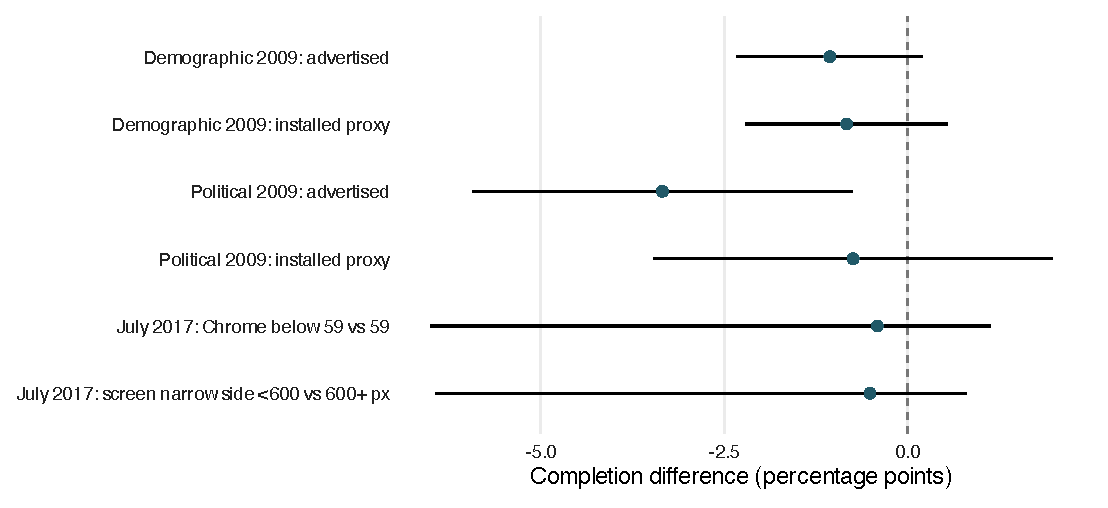
\includegraphics[width=\linewidth]{../figs/question_completion.pdf}
\caption{Completion contrasts answer different technical questions. Points show percentage-point differences and lines show 95\% intervals: HC2 normal intervals for the historical version comparisons and Newcombe intervals constructed from Wilson limits for July 2017. Historical contrasts compare legacy versus other recognized browsers; the installed proxy reclassifies IE8 compatibility records. July contrasts compare earlier versus current desktop Chrome and a recorded screen dimension below 600 pixels on the narrower side versus at least 600 pixels. Each estimate uses its own observed sample. Shared axes compare magnitudes, not a common treatment effect; historical components and alternative definitions reuse respondents.}
\label{fig:participation}
\end{figure}

The July comparisons are much less precise (Table~\ref{tab:july}). Among \ChromeN{} earlier-major desktop Chrome records, completion is \ChromeRate\%, compared with \ChromeReferenceRate\% among \ChromeReferenceN{} current-major records. The gap is \ChromeGap{} points (\ChromeInterval{}). The comparison excludes \ChromeOutsideN{} records outside these two version groups. For records with a screen dimension below 600 pixels on the narrower side, completion is \ResolutionRate\% among \ResolutionN{} records versus \ResolutionReferenceRate\% among \ResolutionReferenceN{} records at or above that threshold. The gap is \ResolutionGap{} points (\ResolutionInterval{}). Neither interval establishes a small effect: both allow an appreciable disadvantage as well as little difference.

\begin{table}[htbp]
\centering
\caption{July 2017 completion differences.}
\label{tab:july}
\small
\begin{tabular}{lrrr}
\toprule
Comparison & $N_1$ & $N_0$ & Gap [95\% CI], points \\
\midrule
Earlier / current Chrome & 72 &  715 & -0.41 [-6.50, 1.13] \\
Screen narrow side: <600 / 600+ px & 74 & 1190 & -0.51 [-6.44, 0.80] \\
\bottomrule
\end{tabular}

\par\smallskip
\begin{minipage}{\linewidth}\footnotesize
\emph{Note}: $N_1$ and $N_0$ are the first and second named groups. Positive differences favor the first group. All unfinished records are retained in the underlying US-coded, consented sample. Intervals use binomial group counts and assume independent responses within this survey; they do not account for selection into MTurk or into the retained export.
\end{minipage}
\end{table}

These are a small set of descriptive comparisons, selected for interpretable measures rather than significance. The historical contrasts use unadjusted differences and HC2 standard errors; the sparse July contrasts use Wilson-based intervals that retain uncertainty when a group has few failures. We report the definitions together and do not regard them as independent confirmations. Further historical specifications, unknown-browser bounds, and computation checks appear in the appendix and replication outputs.

\subsection{Answer provision}

The historical fixed field sets contain few blanks among completers. Both browser-group difference intervals include zero (Appendix Table~\ref{tab:blanks}). That result is narrower than a claim of equal survey quality: these fields cover part of each instrument, and selection into completion remains.

The timer-linked 2017 results show why the questionnaire must accompany the technical paradata (Table~\ref{tab:answers}). In July, \SliderBlanks{} of \SliderItems{} recorded rating opportunities on submitted slider blocks have no numeric rating (\SliderRate\%). These are not all identified omissions: the explicit ``Not Applicable'' option also produces a blank. Other formats record don't-knows as text, while some offer no such option. A contrast of blank cells would conflate these response rules with behavior.

\begin{table}[htbp]
\centering
\caption{Recorded answers on timer-linked submitted blocks.}
\label{tab:answers}
\small
\begin{tabular}{lrrrr}
\toprule
Study / format & People & Item records & Blank (\%) & DK (\%) \\
\midrule
March 2017: Choice + closed probe & 374 & 1,870 & 0.0 & 24.1 \\
March 2017: Choice + open probe & 184 & 916 & 0.1 & 25.8 \\
March 2017: Scale & 502 & 10,040 & 0.0 & 0.0 \\
July 2017: Choice + DK (14K) & 250 & 2,242 & 0.0 & 18.5 \\
July 2017: Numeric slider (24K) & 268 & 2,407 & 18.6 & 0.0 \\
July 2017: Choice + DK (FSR) & 253 & 2,277 & 0.0 & 20.6 \\
July 2017: Choice (IPS) & 251 & 2,253 & 0.0 & 0.0 \\
July 2017: Media wording (RW) & 238 & 2,134 & 0.0 & 0.0 \\
\bottomrule
\end{tabular}

\par\smallskip
\begin{minipage}{\linewidth}\footnotesize
\emph{Note}: Percentages use item records linked to positive submission timers; people count distinct response IDs within each row. Unfinished respondents with such records remain included. March choice rows distinguish open versus closed follow-up probes; the table counts the choice fields, not the probes. March formats cover different numbers of fields. July 24K is a numeric-slider format whose blanks include explicit ``Not Applicable'' selections; 14K and FSR offer textual don't-knows, while IPS and RW do not. DK counts are recognized explicit don't-know text, not an inference about knowledge. Rows differ in content, routing, and response options, so their percentages do not rank format quality.
\end{minipage}
\end{table}

Within the July slider format, the unrecorded-rating share is \SliderNarrowRate\% in the group below the 600-pixel threshold and \SliderWideRate\% in the other group. Only \SliderNarrowN{} and \SliderWideN{} respondents, respectively, contribute timer-linked ratings. This is a useful place to inspect the control and its export behavior, but not evidence that small displays caused missing answers. The outcome combines different actions, the groups are selected, and item observations repeat within respondents. The accompanying tables retain the separate numerators, denominators, and respondent-level any-blank intervals.

\subsection{Open-ended response length}

Respondents with mobile-OS records supplied less text on the two common narrative questions in March (Table~\ref{tab:text}). Their mean was \TextMobileMean{} characters per question among \TextMobileN{} respondents, compared with \TextDesktopMean{} among \TextDesktopN{} desktop-OS respondents. The mobile-minus-desktop difference is \TextGap{} characters (95\% Welch interval \TextInterval{}), using each person's two-question average as one observation. Both pages have positive submit timers and nonblank answers for every retained respondent, so the comparison is about response length rather than skipping these questions. Word counts and log(1 + each person's mean character count) also show shorter responses in the mobile group.

\begin{table}[htbp]
\centering
\caption{Open-ended response length on common March 2017 questions.}
\label{tab:text}
\small
\begin{tabular}{lrrr}
\toprule
Recorded group & People & Mean characters & Median [Q1, Q3] \\
\midrule
Browser: Chrome & 701 & 211.6 & 171.5 [98.5, 265.5] \\
Browser: Edge &  38 & 227.2 & 185.8 [89.9, 277.5] \\
Browser: Firefox & 200 & 234.6 & 196.8 [124.9, 310.6] \\
Browser: IE &  46 & 191.1 & 159.5 [91.2, 222.8] \\
Browser: Safari &  75 & 198.7 & 170.5 [88.8, 256.8] \\
OS: Desktop OS & 980 & 220.0 & 180.0 [103.4, 282.0] \\
OS: Mobile OS &  80 & 149.9 & 136.5 [69.5, 186.0] \\
\bottomrule
\end{tabular}

\par\smallskip
\begin{minipage}{\linewidth}\footnotesize
\emph{Note}: Each observation is one person's mean character count across the immigration and climate-change prompts. Browser and OS rows regroup the same people and must not be added together. Safari combines desktop, iPhone, and iPad labels. Quartiles describe variation between people, not uncertainty in the mean. Text length includes internal spaces and punctuation. All observations are finished survey records; device and browser use were not randomized.
\end{minipage}
\end{table}

Browser-family summaries also reflect device composition. Safari's mean is \SafariTextMean{} characters across all recorded operating systems and \SafariDesktopTextMean{} when restricted to desktop OS. The supplementary tables retain every observed family, desktop-only comparisons, question-specific summaries, and exploratory intervals against Chrome. These do not isolate software effects. The mobile comparison is consistent with greater typing burden, but differences in knowledge, interest, verbosity, or selection into completion could also produce it. For a survey organization, the actionable next test is whether a different text-entry interface increases relevant information on the same questions, assessed separately from word count.

\subsection{Elapsed time}

The recorded duration patterns do not show a uniform mobile-OS disadvantage (Table~\ref{tab:duration}). The mobile and desktop medians are \MarchMobileMinutes{} and \MarchDesktopMinutes{} minutes in March, \JulyMobileMinutes{} and \JulyDesktopMinutes{} in July, and \LucidMobileMinutes{} and \LucidDesktopMinutes{} in Lucid. In Stanford A the mobile median is higher (\StanfordAMobileMinutes{} versus \StanfordADesktopMinutes{} minutes); in Stanford B the medians are close (\StanfordBMobileMinutes{} versus \StanfordBDesktopMinutes{}). The questionnaires and selected populations differ. We therefore compare distributions within a survey and do not average these differences into a device effect.

\begin{table}[htbp]
\centering
\caption{Elapsed minutes by recorded operating-system group.}
\label{tab:duration}
\small
\begin{tabular}{lrlrr}
\toprule
Study & Year & OS group & $N$ & Minutes: median [Q1, Q3] \\
\midrule
March & 2017 & Desktop OS &  980 & 8.3 [6.1, 11.4] \\
March & 2017 & Mobile OS &   80 & 7.6 [6.0, 9.1] \\
July & 2017 & Desktop OS & 1147 & 3.0 [2.3, 3.9] \\
July & 2017 & Mobile OS &  106 & 3.1 [2.3, 3.8] \\
Lucid & 2024 & Desktop OS &  173 & 5.5 [3.9, 8.1] \\
Lucid & 2024 & Mobile OS &  559 & 5.1 [3.7, 7.2] \\
Lucid & 2024 & Unknown &  172 & 1.5 [1.0, 2.8] \\
Stanford A & 2018 & Desktop OS &  744 & 13.9 [10.5, 19.0] \\
Stanford A & 2018 & Mobile OS &  715 & 15.4 [11.6, 20.7] \\
Stanford A & 2018 & Unknown &    1 & 14.9 [14.9, 14.9] \\
Stanford B & 2018 & Desktop OS &  632 & 16.7 [12.8, 22.2] \\
Stanford B & 2018 & Mobile OS &  671 & 16.7 [13.2, 21.8] \\
Stanford B & 2018 & Unknown &    1 & 35.2 [35.2, 35.2] \\
\bottomrule
\end{tabular}

\par\smallskip
\begin{minipage}{\linewidth}\footnotesize
\emph{Note}: Entries are medians and empirical quartiles, not confidence intervals. March, July, and Lucid use finished records; Stanford uses retained records without a screenout flag. Unknown OS is retained as its own group. Durations include interruptions. Counts are records; no independent-person inference is made for these distributions. All-record Stanford and resolution-stratified summaries are available separately.
\end{minipage}
\end{table}

Metadata absence can itself mark a different path through a questionnaire. Lucid has \LucidMetadataMissing{} finished records without its reported browser field, despite retaining a raw user-agent field. The unknown-OS group's median is \LucidUnknownMinutes{} minutes. A finished flag therefore does not guarantee comparable exposure to every questionnaire block. This is a reason to inspect survey flow before attributing the duration pattern to technology or interpreting missing technical paradata as random.

\section{Does the signal add useful information?}

The preceding comparisons describe the available records. They do not establish that technical paradata improve an organization's predictions beyond its panel profiles and participation history. That is a separate empirical question. A signal can be useful for prediction without identifying a technical mechanism, while a statistically distinguishable in-sample association can add little predictive value.

These surveys do not support an adjusted comparison of completion using pre-survey respondent profiles. Every historical political dropout lacks the full demographic control set. July party identification is missing for every unfinished record, and age is missing for most. The additional finished-only samples have no completion variation. Restricting a model to complete demographics would remove the outcome cases of interest, rather than adjust a comparable population. We consequently do not report an adjusted completion coefficient or a predictive validation exercise.

An eligible panel analysis would compare the same held-out records under three information sets: questionnaire information and pre-survey profiles; those variables plus prior participation; and that baseline plus technical paradata. Training would precede the evaluation wave, and later responses would never enter earlier predictions. Calibration, Brier score, and log loss would measure forecast quality. Holding out people would separately test generalization to new panelists. These are different applications from forecasting the next survey for known panelists, and must not be conflated.

Measurement checks are already possible. The public corpus of \JssN{} user-agent records from \JssSurveys{} surveys provides a broad test of whether explicit family tokens can be recognized \citep{rossmann2020}. The corpus does not provide verified fieldwork dates; 2020 is the publication year. Our limited token rules leave \CorpusUnknown{} unresolved. This is coverage, not accuracy against known installations. In Lucid, reported browser labels and resolvable raw strings agree in \ParserAgreement{} records and differ in \ParserDifferent{}; \ParserUnresolved{} raw strings are unresolved when reported labels exist, and \ParserMissing{} records lack reported labels. Differences can reflect detection rules, collection points, or configuration changes. Neither field is ground truth. An organization should validate its detector and the timing of metadata collection before depending on the signal.

\section{What could a survey organization do with the signal?}

The immediate use is to narrow an investigation. In the historical survey, compatibility settings deserve attention because the completion contrast changes substantially when their meaning changes. In July, the slider's export rules deserve attention because a blank can record an explicit answer. In Lucid, technical-field absence warrants a survey-flow check. These examples identify questions for a survey organization; they do not show that a browser upgrade or layout change would recover the observed losses.

The operational response depends on the use. For diagnosis, locate the page and configuration where problems concentrate, reproduce the questionnaire under that configuration, and inspect requests, errors, and rendering. For forecasting, require gains in later surveys beyond existing profiles and history. For delivery, test simpler grids, lighter pages, or alternative controls while holding content and incentives fixed. Before using answer length to score engagement, validate its relationship with independent measures of interest or relevant behavior across technical environments. Prioritization should consider both the prevalence of a configuration and the size of its observed gap; rare configurations with large gaps and common ones with modest gaps can imply different testing priorities. An observational gap is not a count of recoverable completions.

For sample composition, compare pre-survey profiles of starters and completers. A remedy may change composition as well as the number of responses. Higher completion alone does not establish reduced population bias. Browser metadata should not be used to exclude respondents merely because their configuration predicts difficulty, and an association alone does not justify a new weighting adjustment.


A suspected interface problem calls for direct observation. Compatibility checks can establish whether a control renders, accepts input, and saves the intended answer. Task-based usability sessions can then reveal where respondents struggle to enter text, select a rating, or recover from an error \citep{moran2019}. For open-ended questions, a fixed-text entry task would isolate input demands from differences in what respondents know; a separate substantive prompt would test answer production. Neither test alone establishes an effect on survey completion.

Once a specific problem and remedy are identified, randomly assign the existing or revised interface while holding wording, response options, and incentives fixed. Assignment before the affected page and retention of every assigned respondent would support a comparison of subsequent completion. Relevant content, answer length, and effort should be measured separately: more characters need not mean better answers. Pre-survey profiles would permit a composition analysis. This design tests whether changing the interface improves survey performance; the browser associations identify where to investigate.

\begingroup
\small
\setstretch{1}
\bibliographystyle{plainnat}
\bibliography{references}
\endgroup
\clearpage
\appendix
\section*{Appendix: Measurement and reproducibility}
\addcontentsline{toc}{section}{Appendix: Measurement and reproducibility}
\subsection*{Historical measurement and reproduction}

The original script classifies browsers by scanning punctuation-stripped strings for broad substrings, including \texttt{98}, \texttt{iphone}, and \texttt{firefox30}. That rule can match unrelated digits, mistake a secondary Internet Explorer token for the primary one, and miss older Firefox versions. The revised historical parser reads explicit version tokens and preserves unknowns. The full specification comparison is shown in Figure~\ref{fig:historical}; all definitions are exploratory sensitivities using overlapping records.

\begin{figure}[htbp]
\centering
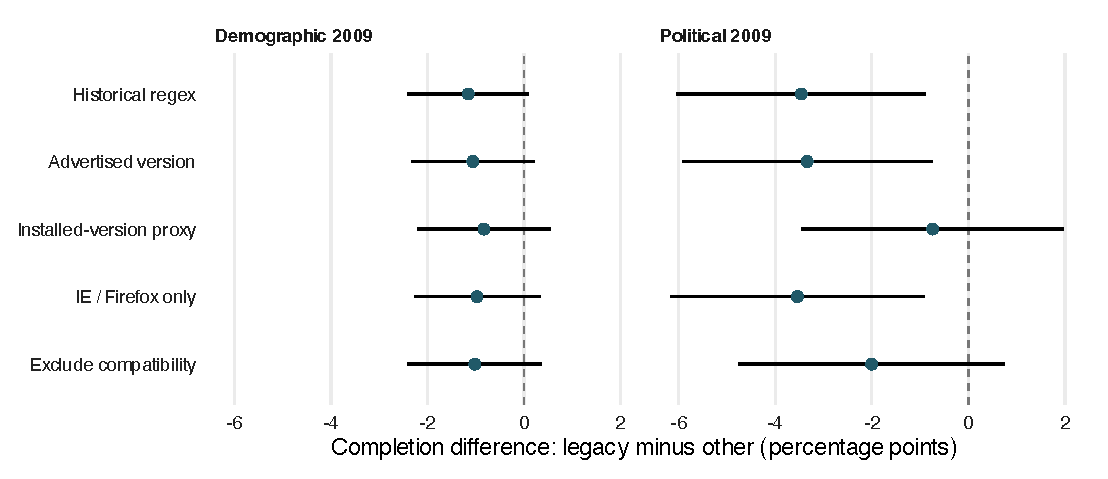
\includegraphics[width=\linewidth]{../figs/completion.pdf}
\caption{Historical completion differences under alternative browser definitions. Points compare legacy and comparator completion; lines show 95\% HC2 normal intervals. Each survey component uses its own observed starters. Unknown strings are excluded except under the historical regex. The panels are dependent samples.}
\label{fig:historical}
\end{figure}

The original SPSS exports confirm the source identities and every linked status and trimmed user-agent value. They establish that the demographic component is \texttt{.x} and the political component is \texttt{.y}; the earlier note reversed those labels. The older README's December--January invitation account does not match the October field timestamps. Invitation totals and population representativeness cannot be established from this extract. These provenance corrections do not supply missing pre-survey demographic information.

The original missing-data outcome counts \texttt{NA} cells across all \MergedColumns{} merged-file columns, mixing routing, absent components, metadata, experimental branches, and derived fields. It excludes empty strings. The revised fixed-field outcome is therefore a different quantity, not simply a corrected estimate of the same construct. Table~\ref{tab:blanks} reports the limited fixed-field sensitivity among completers.

\begin{table}[htbp]
\centering
\caption{Fixed-field blanks among historical survey completers.}
\label{tab:blanks}
\small
\begin{tabular}{lrrrrrr}
\toprule
Survey & Year & Fields & $N$ & Legacy & Other & Difference [95\% CI] \\
\midrule
Demographic & 2009 & 9 & 2009 & 0.003 & 0.002 & 0.002 [-0.004, 0.007] \\
Political & 2009 & 5 & 2055 & 0.005 & 0.011 & -0.006 [-0.015, 0.003] \\
\bottomrule
\end{tabular}

\par\smallskip
\begin{minipage}{\linewidth}\footnotesize
\emph{Note}: Means count blank fields per person, including whitespace-only text. Explicit don't-knows count as recorded answers. Demographic fields cover handedness, state, gender, household composition, birth month/year, marital status, education, and Hispanic origin; political fields are the knowledge questions. Intervals use HC2 standard errors. Unknown browser versions are excluded. Question-level exposure is unverified, so these are not all-question item-nonresponse rates.
\end{minipage}
\end{table}

The 2023 adjusted missing-cell models retain the same \HistoricalMissingN{} people and return the same browser coefficient, \HistoricalMissingGap{} ($p=\DemMissingP{}$). The 2011 models instead use different samples and duration restrictions. Their completion tests reproduce $p=\DemNoteP{}$ and $p=\PolNoteP{}$; the 2023 completion tests give $p=\DemOldP{}$ and $p=\PolOldP{}$. These are specification changes rather than a failure to reproduce the earlier arithmetic.

\subsection*{Checks and reproducibility}

For a two-group mean difference, HC2 variance equals the sum of the two sample variances divided by their group sizes \citep{sandwich}. Independent arithmetic checks, alternative logistic summaries, Fisher tests, deletion influence, and all allocations of unknown browser statuses are in the replication outputs. Seeded simulations assess interval behavior under independent Bernoulli sampling, not the sample's representativeness. Sparse July differences use Newcombe intervals derived from Wilson limits, checked independently from their group counts. The duration quartiles are descriptive distribution summaries rather than uncertainty intervals. For March narrative responses, we average the two common questions within each person before computing Welch intervals from group means and variances. Browser-family intervals are exploratory and unadjusted for multiple comparisons; word counts, log-transformed person means, question-specific summaries, and single-record deletion bounds are retained in the replication outputs.

The expanded analysis keeps source-specific imports separate from the shared technical and outcome definitions. The item/timer map, source hashes, duplicate checks, measurement ledger, and retrospective analysis plan are recorded in the repository. Source imports write aggregate summaries only. The ordinary build regenerates question-organized tables, figures, and manuscript numbers from the historical data and those aggregates; rebuilding the aggregate snapshots requires the authorized sibling exports and downloaded public corpus.

\end{document}
